\documentclass[pdftex,12pt,a4paper]{article}

% just for this template
\usepackage{lipsum}

% For graphics
\usepackage[pdftex]{graphicx}
% you can place a figure at the position where it occurs in the text using [H]
\usepackage{here}

% For flexible tables
\usepackage{multirow}

% In case you need umlauts
% \usepackage[utf8]{inputenc}


% Sophisticated citation.
% Check out: http://merkel.zoneo.net/Latex/natbib.php
\usepackage{natbib}

% Math symbols not defined in the usual package, e.g. arrows that are crossed.
\usepackage{amssymb}

% Arrows with text / superscript
\usepackage{amsmath}

% Different font - something like Arial
%\usepackage{mathptmx}

% Adjust margin of paper.
\usepackage{geometry}
\geometry{a4paper, top=25mm, left=25mm, right=25mm, bottom=25mm}

% Zeilenabstand 1.25 %
\linespread{1.2}

% Example Environments
\usepackage{amsthm}
\newtheoremstyle{style}   
  {0.5cm}              %Space above    
  {-0.8cm}              %Space below
  {}                      %Body font: original {\normalfont}    
  {}                      %Indent amount (empty = no indent,%\parindent = paraindent)    
  {\normalfont\bfseries}  %Thm head font original       
  {{\normalfont\bfseries \thmname{#1}\thmnumber{ #2}}}
\theoremstyle{style}
\newtheorem{example}{Example}[section]

% Formula Environments
\newtheorem{formula}{Formula}[section]

% Computational Linguistics trees etc.
\usepackage{xyling}

% Nicer captions
\usepackage{caption2}
\newcaptionstyle{mystyle}{%
  \normalcaptionparams
  \renewcommand\captionlabelfont{\bfseries}%
  \renewcommand\captionlabeldelim{.}%
  \onelinecaptionsfalse
  \usecaptionstyle{centerlast}}

\captionstyle{mystyle}

% Table of contents depth
\setcounter{tocdepth}{3}

% A horizontal rule for the title page
\newcommand{\HRule}{\rule{\linewidth}{0.5mm}}

% Paragraph and indent (as required by Prof. Dr. Pinkal)
\setlength{\parindent}{0pt}
\setlength{\parskip}{2ex plus 0.5ex minus 0.2ex}

\begin{document}

% Include the title page (modify title.tex!)
\begin{titlepage}
\begin{center}

% Upper part of the page. The '~' is needed because \\
% only works if a paragraph has started.

\includegraphics[width=0.25\textwidth]{./eule}~\\[1cm]

\textsc{\LARGE Saarland  University}\\[0.4cm]
\textsc{\Large Department of Language Science and Technology}\\[1.5cm]

\textsc{\Large Software Project Report:} \textbf{\Large Natural Language Processing with Neural Networks}\\[0.5cm]

% Title
\HRule \\[1.0cm]

{ \huge \bfseries Proto-Word Reconstruction using Neural Networks}\\[0.4cm]

\HRule \\[1.5cm]

% Author and supervisor
\begin{minipage}{0.4\textwidth}
\begin{flushleft} \large
\emph{Authors:}\\
Julius \textsc{Steuer}\\
Matriculation: 2576077
Morgan \textsc{Wixted}\\
Matriculation: 2576217
\end{flushleft}
\end{minipage}
\begin{minipage}{0.4\textwidth}
\begin{flushright} \large
\emph{Guided by:} \\
Prof. Dr. Dietrich \textsc{Klakow}\\
\end{flushright}
\end{minipage}

\vfill

% Bottom of the page
{\large \today}

\end{center}
\end{titlepage}


\thispagestyle{empty}
\begin{abstract}
\setlength{\parskip}{2ex plus 0.5ex minus 0.2ex}

% Please put \noindent before each paragraph of the abstract!
\noindent 
Reconstructing a proto language requires large amounts of cognate data. In recent years automated approaches to proto-word reconstruction have been introduced that try to establish these relationships without relying on human knowledge. One of these approaches is using a decoder-encoder neural model with attention.
In our paper, we evaluate whether a decoder-encoder model is necessary to weigh the influence of the individual languages on the form of the reconstructed word. We test a series of simpler (recurrent and non-recurrent) models on a dataset that is often used for this purpose. In addition, we compile a smaller data set to evaluate how these models scale to low-researched families. 
We found that all models tested performed worse compared to a sequence-to-sequence baseline in \citet{meloni2019ab}, with simple recurrent and LSTM recurrent models being outperformed by a deep feedforward model. In addition we observed a signifcant drop in performance when training on the self-compiled dataset, indicating that large cognate data sets are required for the task.
\end{abstract}
\newpage

% Table of contents
\thispagestyle{empty}
\tableofcontents
\newpage

% Start of content
\setcounter{page}{1}		% Seitenzähler auf 1 setzen %
%\pagestyle{fancy}				% fancy header style
\pagenumbering{arabic}
\newpage
\section{Introduction}

Recent approaches on the automated reconstructions of proto-words made use of phylogenetic methods, for example, \citet{bouchard-Cote_et_al:2013} for Austronesian
and \citet{hruschka_detecting_2015} for Turkic. Another approach is to use a neural decoder-encoder model with attention, a pipeline used in machine translation, to map sequences of cognate sounds
in related words to a single sound in the (supposedly unknown) parent language. Examples of this approach are \citet{ciobanu-dinu-2018-ab} and \citet{meloni2019ab}.
While the phylogenetic approaches rely on phonological features of the sounds involved to reconstruct proto-words (and to derive the most likely family tree), 
the latter two make use of character embeddings to represent sounds. In contrast, \citet{dekker_msc_2018} uses a neural machine translation model in conjunction with feature encodings. 

How plausible is using a machine translation pipeline for automatically resontructing proto-words? While a machine translation system maps a sequence of words in one language onto a sequence of words in another language (while preserving the meaning), the above approaches map a sequence of sounds or characters pertaining to a word in a cognate set to a single sound in the proto-language. Since sounds do not make up the meaning of a word in the same sense as words make up the meaning of a sentence (with every word contributing an identifiable part to it), we suspect that a more simple recurrent or even non-recurrent architecture may as well capture sound correspondences. 

Another feature of the above approaches is that they seem not to benefit from more a more fine-grained transcription: if IPA transcriptions are used as input to a model, reconstruction accuracy is always lower compared to the ordinary Latin orthography.
We will investigate whether a more coarse transcription as that used in the context of the ASJP database \cite{brown_automated_2008} does improve reconstruction accuracy.
% On the other hand, having fewer datapoints to reconstruct automatically reduces the error

Finally, we want to explore how automatic methods can be applied to smaller datasets, and to language families for which the proto-language is not well established. We therefore compiled a custom romance dataset and compare the performance of our models on it to their performance with a dataset used in the prior studies.

\newpage
\newpage

\subsection{Literature Review}
%-----------------------------------------------------------------------------------------------------
%--- Literature
%-----------------------------------------------------------------------------------------------------
%\section{Background}
Recent approaches on the automated reconstructions of proto-words made use of phylogenetic methods, see \cite{bouchard-Cote_et_al:2013} for Austronesian
and \cite{hruschka_detecting_2015} for Turkic. Another approach is to use a neural machine translation pipeline with attention to map sequences of cognate sounds
in related words to a single sound in the (supposedly unknown) parent language. Examples of this approach are \cite{ciobanu-dinu-2018-ab} and \cite{meloni2019ab}.
While the phylogenetic approaches rely on phonological features of the sounds involved to reconstruct proto-words (and to derive the most likely family tree), 
the latter two make use of character embeddings to represent sounds. In contrast, \cite{dekker_msc_2018} used a neural machine translation model in conjunction with feature encodings. 
%-----------------------------------------------------------------------------------------------------
%--- Data
%-----------------------------------------------------------------------------------------------------

\section{Methods}
\subsection{Data}
\begin{table*}
\centering
\begin{tabular}{lcc}
    \hline
    & \textbf{I} (Swadesh list) & \textbf{II} (Ciobanu 2014) \\
    \hline
    \textbf{Languages} & \multicolumn{2}{c}{Italian, Spanish, French, Portuguese, Romanian} \\
    \textbf{Ancestor} & \multicolumn{2}{c}{Latin} \\
    \textbf{Size} & 100 & 3218 \\
    \textbf{Train set} & 80 & 2574 \\
    \textbf{Test set} & 20 & 644 \\
    \textbf{Aligned} & yes & no \\
    \textbf{Alphabets} & \multicolumn{2}{c}{IPA, ASJP, Latin} \\
    \hline
\end{tabular}
\caption{Datasets}
\label{tab:datasets}
\end{table*}

%\subsubsection{Alphabets}
\subsubsection{Alphabets \& self-compiled dataset}
We compile cognate sets based on the Swadesh lists \cite{swadesh_origin_1971} for the 5 romance languages used in \citet{ciobanu-dinu-2014-automatic} (Italian, Spanish, French Portuguese \& Romanian) using two
different alphabets: The International Phonetic Alphabet (IPA) and the alphabet of the Automated Similarity Judgment Program (ASJP). The datasource was for the most part the etymological section of the Wiktionary \footnote{https://www.wiktionary.org}.
The ASJP alphabet comprises all ASCII characters and is used primarily for phylogenetic inference. The advantage of using the ASJP alphabet in addition to IPA is that wordlists containing 40 or 100 words from the Swadesh list are available for many language families, and likely the first data collected for
any unknown language. Also, the feature set contained in ASJP is less fine-grained than that of IPA, describing sound classes rather than individual sounds

\begin{figure}
\centering
$\begin{pmatrix}
    k & a & p & u & - & - \\
    k & a & p & o & - & - \\ 
    k & a & b & e & 8 & a \\
    S & E & f & - & - & - \\
    k & a & b & u & - & - \\
    & k & a & p & - & - & - 
\end{pmatrix}$
\label{figure:alignment}
\caption{Aligned item 38 (HEAD) from Swadesh data. \{-\} are placeholder tokens indicating either loss in one or innovation in another daughter language.}
\end{figure}

We also added manually aligned cognate sets to our self-compiled data in order to investigate whether introduction of top-down knowledge, i. e. hypotheses about the relationships between the sounds in the daughter languages improve the quality of reconstructions. \ref{figure:alignment} shows the manual alignment for item 38 from the Swadesh list. 

Since the feature values of the individual
characters are not fixed, we use those given in \cite{brown_automated_2008}.
From these alphabets, we derived multi-hot
embeddings based on the phonological features of a sound represented by a character of either alphabet, and one-hot character embeddings from the surface characters.That means that each character is once encoded as a vector of [0, 1] for each phonological feature, and once as one row in a identity matrix 
where rows and columns represent the characters of the alphabet. 

Since Latin is not the direct ancestor of the romance languages, and none of the languages our dataset
actually continues (e. g.) the Latin nominative in nouns or the passive inflection in verbs, we chose
to replace the Latin lemma form with either the stem of the accusative singular in nouns or the "active"
infinitive in verbs. This deviates from all prior approaches, but since it is well established that Classical Latin
is not the direct ancestor of the romance language family (compare \citet{Dworkin_2016}), and most lemmas in the individual languages
do not continue (e. g.) the Latin nominative or infinitive, we decided to use a form that more closely matches the actual
ancestor of the romance words. Therefore, we replaced Latin \textit{pe:s} with a normalized accusative singular \textit{*pede},
and a passive infinitive as \textit{mori:} with its active counterpart \textit{*mori:re}, which is the ancestor of Spanish \textit{morir}, 
French \textit{mourir} etc. We think that this approach is valid since no romance language actually preserves the nominative form,
which therefore should be impossible to reconstruct if only the romance data is known.

\subsubsection{Dataset from \citet{ciobanu-dinu-2014-automatic}}
We also test our model on a larger dataset. We chose the romance data provided by \citet{ciobanu-dinu-2014-automatic} because it was used by
\citet{meloni2019ab}. One drawback of this dataset is that it consists mainly of direct loans from Latin, which in addition to the conservative spelling
conventions makes it somewhat artificial compared to data that is collected from oral sources where no transcription is available. We want to circumvent this
drawback by using our smaller dataset containing cognate sets that actually mirror the phonological developments leading to the modern languages.
This is different from phylogenetic approaches where loans serve the goal of the reconstruction, i. e. reconstructing a family tree that mirrors language contact.
Since we want to reconstruct proto-words and we opted to have only some aberrant items that represent either loans from Latin or lexical replacement.

As a baseline, we also compiled a latin alphabet version of our dataset to test our models under the same conditions as in \citet{meloni2019ab}.


%-----------------------------------------------------------------------------------------------------
%--- Models
%-----------------------------------------------------------------------------------------------------
\begin{table*}
\centering
\begin{tabular}{ccc}
    \hline
    % @Morgan: add the RNN model here?
    & \textbf{A} & \textbf{B} \\
    \hline
    \textbf{Architecture} & Recurrent & Deep feedforward \\
    \textbf{Hidden layer} & LSTM layer & 2 dense layers \\
    \textbf{Size} & 128 & 2 $\times$ 256 \\
    \hline
    & 
\end{tabular}
\caption{Models}
\label{tab:my_label}
\end{table*}

\subsection{Models}
Here we discuss the different models we use to reconstruct the proto-words.
We use several different models to evaluate how well they reconstruct each proto-word, given a cognate set. We use a simple recurrent neural network (RNN), a long short-term memory (LSTM) network, and a deep feedforward neural network with two hidden layers.\\
For both the RNN and the LSTM, we use the stochastic gradient descent algorithm for optimization. For the deep feedforward neural network, we use the Adam algorithm for optimization.\\
% Say something about batching? We didn't do it with the swadesh data because the dataset was small,
% but it might have been a good idea for the ciobanu data after all...
As for the loss function, each network uses cosine similarity. This is because we are wanting to measure the similarity between each character of each derived language in comparison to the character of the reconstructed proto-word in question. We also retrieve the reconstructed character from the alphabet by calculating cosine similarity with the feature or embedding vector. \\
% JS: if we say statistically significant we should actually perform some tests^^
For the parameters, in our experiments, any value lower than 128 produced worse results. Any value much higher than 128 (for example, 160), also produced worse results. A lower value, such as 150, produced slightly better results, but not enough to be statistically significant. Therefore, we use the default parameters provided by Tensorflow for our models.

We trained each model for 10 epochs. Using a higher number of epochs improved edit distance scores for dataset \textbf{A}, but not for dataset \textbf{B}. Since the former contains much less items than the former, training our models over more epochs would only lead to overfitting, thus we decided to have an equal number of epochs for both datasets.

\subsubsection{Simple Recurrent Neural Network}
To construct our simple recurrent neural network, we use the Keras Application Program Interface (API) \cite{chollet2015keras} from Tensorflow \cite{tensorflow2015-whitepaper}. Following the example from Tensorflow, we use a sequential model consisting of an embedding layer, a simple recurrent neural network layer, and a dense layer. \\
As for parameters, the only parameter that can be tuned is the context dimension, how many units the RNN has. Tensorflow has a default value of 128 for the context dimension. 

\subsubsection{Long Short-Term Memory Neural Network}
To construct our long short-term memory neural network, we again use the Keras API from Tensorflow. As we did with the RNN, we also follow the example that Tensorflow gives. We use a sequential model consisting of an LSTM layer that takes five inputs (consisting of the five characters of each of the romance languages), two dense layers: one to avoid narrowing of the signal from 128 to 10 in one step and another to represent the size of the character embedding. 

\subsubsection{Deep Feedforward Neural Network}
To construct our deep feedforward neural network, we use Keras. In contrast with our RNN and LSTM models, we manually construct this network instead of using an API. The network is constructed by creating five hidden dense layers (for each romance language), flattening the layers to create one all-encompassing layer, and then having a final dense layer as the output. 

\subsection{Thoughts on our models and data}
Our experiments could use some improvements, especially with the evaluation. Our current evaluation metrics have the average edit distance normalized by word length. This means that each error carries the same weight regardless of where it occurs in the word. 
We think that errors that occur in the stem would be more grave than if they occurred in the suffix, therefore, errors in the steam of the word should carry a larger weight than errors in the suffix of the word. 
As another example, reconstructed words that differ by only one phoneme. Say we have $/t$ and $/d/$. These phonemes only differ by their voicing, so this error should not be greatly penalized. Ideally, we would have a list of criteria that could be used to penalize errors appropriately during evaluation.
Additionally, we should have replicated the baseline from \cite{meloni2019ab}, but we did not.

\subsection{Training}
\subsubsection{Loss}

\begin{figure}
    \centering
    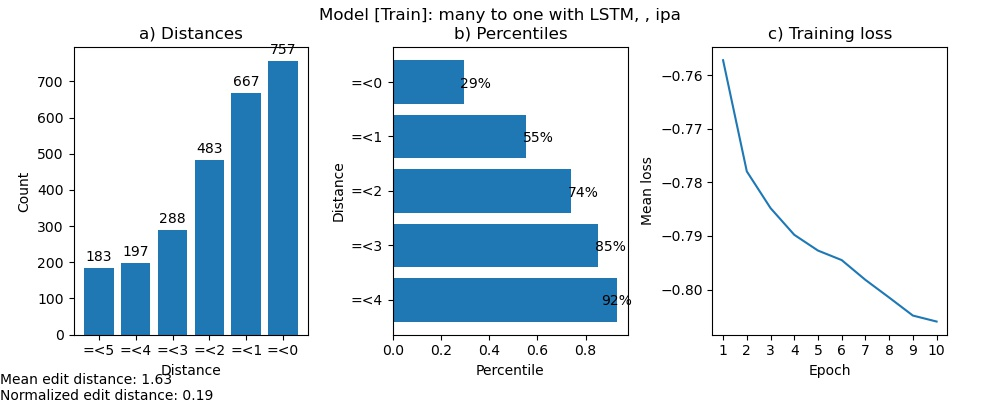
\includegraphics[width=\textwidth]{many2one_train_ipa.jpg}
    \caption{Train loss and edit distances for model A on data set II}
    \label{fig:loss_curve}
\end{figure}
We observed that the average per-batch accumulate loss over all epochs seems to approach -1 (compare \ref{fig:loss_curve}). This might be because we use cosine similarity as a loss function, which takes values in $[0,1]$. Assuming that the similarity between the output layer of the network and the ground truth vector is random, one would expect cosine similarity to be close to 0. Over training cosine similarity increases and ideally approaches 1, meaning that the total loss available is also close to 1.

\subsubsection{Activation Function}
As mentioned above we used sigmoid as the activation function on the final layers, since the ground truth vectors representing the character features/embeddings were distributed multi-hot/one-hot vectors. However, in the case of character embeddings our pipeline comes close to a classification task, with the ground truth vector having a 1 at the location of the true character and a 1 everywhere else. Therefore we could also use softmax as the activation function on the output layer,deriving a probability distribution over the set of characters. We retrained our best-performing model (\textbf{II}) for dataset \textbf{A}, with performance being slightly worse.

%-----------------------------------------------------------------------------------------------------
%--- Results
%-----------------------------------------------------------------------------------------------------
\newpage
\section{Results}
We report edit distance percentiles, mean edit distance and the mean edit distance normalized for word length for each test condition. An edit distance of 0 means that the reconstructed word differed in 0 characters from the ground truth, i. e. a perfect reconstruction. We do not include the results for the simple recurrent model since it was consistently outperformed by the LSTM model. Additionally, we did not replicate the baseline from \cite{meloni2019ab}, so see there for a comparison with our models.

% Results on swadesh dataset
\begin{table*}
\centering
\begin{tabular}{c|c|c|ccccc|cc}
    \hline
    \multicolumn{3}{c|}{\textbf{Model}} & \multicolumn{5}{c|}{\textbf{Edit Distance}} & \textbf{Mean} & \textbf{Norm} \\
    \multicolumn{3}{c|}{} & \textbf{$\leq$} 0 & \textbf{$\leq$} 1 & \textbf{$\leq$} 2 & \textbf{$\leq$} 3 & \textbf{$\leq$} 4 & \\
    \hline
    
    % Feature encodings
    \multirow{4}{*}{\textbf{Features}} 
        & \multirow{2}{*}{\textbf{IPA}} 
            &  \textbf{A} & 12\% & 35\% & 59\% & 76\% & 87\% & 2.31 & 0.37 \\
            && \textbf{B} & 15\% & 41\% & 61\% & 78\% & 84\% & 2.21 & 0.35 \\
        \cline{2-10}
        & \multirow{2}{*}{\textbf{ASJP}}
            &  \textbf{A} & 21\% & 55\% & 73\% & 87\% & 92\% & 1.72 & 0.3 \\
            && \textbf{B} & 28\% & 54\% & 76\% & 89\% & 92\% & 1.59 & 0.27 \\
    \hline
    
    % Character embeddings
    \multirow{4}{*}{\textbf{Orthographic}} 
        & \multirow{2}{*}{\textbf{IPA}} 
            &  \textbf{A} & 29\% & 41\% & 65\% & 78\% & 92\% & 2.05 & 0.44 \\
            && \textbf{B} & 14\% & 33\% & 62\% & 79\% & 91\% & 2.21 & 0.45 \\
        \cline{2-10}
        & \multirow{2}{*}{\textbf{ASJP}}
            &  \textbf{A} & 31\% & 52\% & 72\% & 85\% & 93\% & 1.67 & 0.29 \\
            && \textbf{B} & 30\% & 51\% & 77\% & 90\% & 94\% & 1.58 & 0.28 \\
    \hline
    
    % Manual alignments
     \multirow{4}{*}{\textbf{Aligned}} 
        & \multirow{2}{*}{\textbf{IPA}} 
            &  \textbf{A} & 9\% & 28\% & 46\% & 73\% & 81\% & 2.6 & 0.44 \\
            && \textbf{B} & 9\% & 22\% & 48\% & 69\% & 84\% & 2.68 & 0.35 \\
        \cline{2-10}
        & \multirow{2}{*}{\textbf{ASJP}}
            &  \textbf{A} & 16\% & 38\% & 57\% & 76\% & 90\% & 2.22 & 0.42 \\
            && \textbf{B} & 21\% & 43\% & 59\% & 81\% & 92\% & 2.04 & 0.39 \\
    \hline
    
     % Manual alignments & character embeddings
     \multirow{4}{*}{\textbf{\begin{tabular}{c} Aligned \\ \& \\ Orthographic \end{tabular}}}
        & \multirow{2}{*}{\textbf{IPA}} 
            &  \textbf{A} & 11\% & 25\% & 43\% & 69\% & 84\% & 2.68 & 0.46 \\
            && \textbf{B} & 11\% & 26\% & 44\% & 72\% & 83\% & 2.64 & 0.47 \\
        \cline{2-10}
        & \multirow{2}{*}{\textbf{ASJP}}
            &  \textbf{A} & 15\% & 35\% & 56\% & 77\% & 87\% & 2.3 & 0.45 \\
            && \textbf{B} & 11\% & 37\% & 57\% & 82\% & 93\% & 2.19 & 0.41 \\
    \hline
    
    % Latin
    \multicolumn{2}{c|}{\multirow{2}{*}{\textbf{Latin}}}
        &  \textbf{A} & 20\% & 37\% & 66\% & 84\% & 87\% & 2.07 & 0.36 \\ % Better performance of Latin orthography only observable in the ciobanu dataset (more data, loans are more likely to preserve the structure of the proto-language)
        && \textbf{B} & 18\% & 39\% & 62\% & 86\% & 94\% & 2.01 & 0.34 \\
    \hline
\end{tabular}
\caption{Performance of both models on the test set of dataset \textbf{I}, 5 cross-validation folds}
\label{tab:results_swadesh}
\end{table*}

% Results for Ciobanu dataset
\begin{table*}[!b]
\centering
\begin{tabular}{c|c|c|ccccc|cc}
    \hline
    \multicolumn{3}{c|}{\textbf{Model}} & \multicolumn{5}{c|}{\textbf{Edit Distance}} & \textbf{Mean} & \textbf{Norm} \\
    \multicolumn{3}{c|}{} & \textbf{$\leq$} 0 & \textbf{$\leq$} 1 & \textbf{$\leq$} 2 & \textbf{$\leq$} 3 & \textbf{$\leq$} 4 & \\
    \hline
    
    % Feature encodings
    \multirow{4}{*}{\textbf{Features}} 
        & \multirow{2}{*}{\textbf{IPA}} 
            &  \textbf{A} & 23\% & 49\% & 67\% & 83\% & 90\% & 1.85 & 0.21 \\
            && \textbf{B} & 29\% & 54\% & 69\% & 83\% & 90\% & 1.72 & 0.2  \\
        \cline{2-10}
        & \multirow{2}{*}{\textbf{ASJP}}
            &  \textbf{A} & 25\% & 50\% & 66\% & 81\% & 90\% & 1.85 & 0.22 \\
            && \textbf{B} & 30\% & 53\% & 69\% & 83\% & 91\% & 1.71 & 0.2  \\
    \hline
    
    % Character embeddings
    \multirow{4}{*}{\textbf{Orthographic}} 
        & \multirow{2}{*}{\textbf{IPA}} 
            &  \textbf{A} & 26\% & 49\% & 70\% & 83\% & 91\% & 1.79 & 0.21 \\
            && \textbf{B} & 30\% & 54\% & 71\% & 83\% & 92\% & 1.68 & 0.2 \\
        \cline{2-10}
        & \multirow{2}{*}{\textbf{ASJP}}
            &  \textbf{A} & 29\% & 52\% & 69\% & 85\% & 91\% & 1.71 & 0.2  \\
            && \textbf{B} & 28\% & 53\% & 70\% & 84\% & 91\% & 1.71 & 0.2  \\
    \hline
    
    % Latin
    \multicolumn{2}{c|}{\multirow{2}{*}{\textbf{Latin}}}
        &  \textbf{A} & 27\% & 56\% & 74\% & 87\% & 93\% & 1.6 & 0.19 \\
        && \textbf{B} & 34\% & 63\% & 79\% & 89\% & 92\% & 1.39 & 0.16 \\
    \hline
    
\end{tabular}
\caption{Performance of both models on the test set of dataset \textbf{II}}
\label{tab:results_ciobanu}
\end{table*}

\subsection{Effect of NN Architectures}
The deep feedforward model (model\textbf{B}) achieved the overall best results, with the average normalized edit distance being slightly lower than with the LSTM model. The simple RNN model yielded far higher edit distances over all test conditions. This behaviour is expected since the change in the hidden state in the simple RNN model is only modulated by the model parameters, whereas the LSTM unit in model \textbf{B} determines how much of the last hidden state is kept.

\subsection{Effect of Encoding Schemes}
We did not observe a clear difference in model performance over different encoding schemes, with a slight advantage for orthographic embeddings for the IPA embeddings. The best average normalized edit distance was achieved for the orthographic ASJP embeddings. Using Latin character embeddings resulted in the lowest edit distances on data set \textbf{II}, with edit distances on data set \textbf{II} being slightly higher than those for ASJP feature encodings.
Differences between the two alphabets used are small, with ASJP feature encodings generally yielding lower edit distances than their IPA counterparts.

\subsection{Effect of Manual Alignments}
The performance on the manually aligned version of data set \textbf{I} was generally worse compared to the non-aligned version across all test conditions. 
Using manual alignments alongside orthographic embeddings resulted in even higher normalized edit distances, indicating that both manual alignements and orthographic embeddings increase the complexity of the data.

\subsection{Performance on Data Sets}
We observed the largest difference in model performance across the two data sets. All models consitently yielded higher average normalized edit distances for our self-compiled data set (data set \textbf{I}). This is in line with our expectations since most items in data set \textbf{II} represent direct loans from Latin. Comparing item 156 from data set \textbf{II} with item 15 of data set \textbf{II} it becomes clear that finding the correct Latin form is much harder for the latter.

\begin{tabular}{cc|cccccc}
     \textbf{Data set} & \textbf{Item} & Latin & Italian & Spanish & French & Portuguese & Romanian \\
     \hline
     \textbf{I} & \textbf{15} & parvu & parvo & pequeno & petit & pequeno & mik \\
     \textbf{II} & \textbf{156} & antiquariu & anticuario & antiquário & antichar & antiquario & anticar  
\end{tabular}

\subsection{Summary}

Generally speaking the feedforward model (model \textbf{B}) yields slightly better results than the recurrent model (model \textbf{A}). However the effect is stronger in the data from \citet{ciobanu-dinu-2014-automatic}, with the lowest average edit distance being 1.39 for the latin with model \textbf{A} opposed to 1.6 with model \textbf{B}. Our self-compiled data set \textbf{I} proved harder for either model, with edit distances being on average one character higher than for dataset \textbf{II}.
Differences in model performance for the two alphabets were small, with performance on the IPA alphabet being slightly worse than performance on the ASJP alphabet, in line with the results of \citet{meloni2019ab}. This effect is strongest for data set \textbf{II}. Orthoghraphic (one-hot) encodings did not influence model performance significantly, though the runs with the Latin alphabet on model \textbf{A} on dataset \textbf{II} produced the best overall results. 
Contrary to our intuition there is no clear tendency as to whether manual alignments increase reconstruction accuracy. However, in the ASJP condition mean edit distances are smallest for the aligned data.

% Deep, Swadesh
\begin{figure}
    \centering
    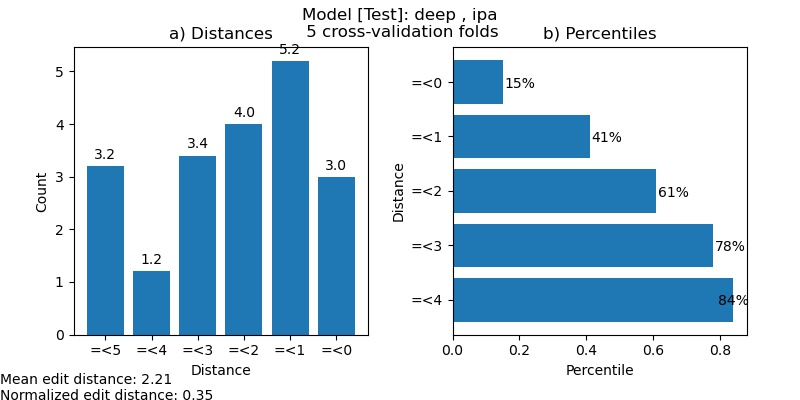
\includegraphics[width=\textwidth]{deep_test_ipa.jpg}
    \label{fig:sdti}
\end{figure}

\begin{figure}
    \centering
    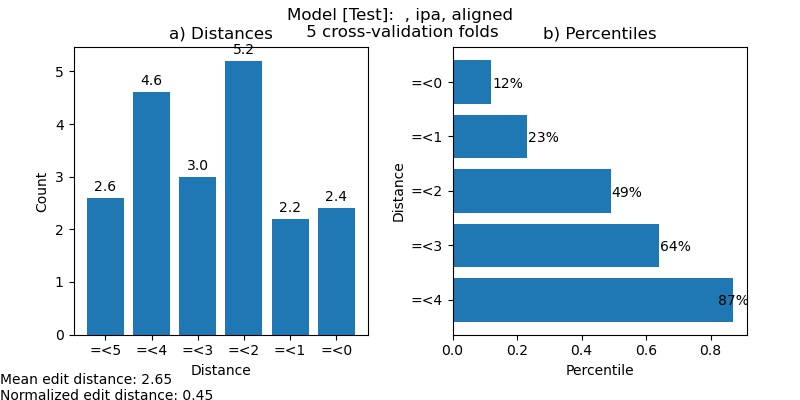
\includegraphics[width=\textwidth]{deep_test_ipa_aligned.jpg}
    \label{fig:sdtia}
\end{figure}

\begin{figure}
    \centering
    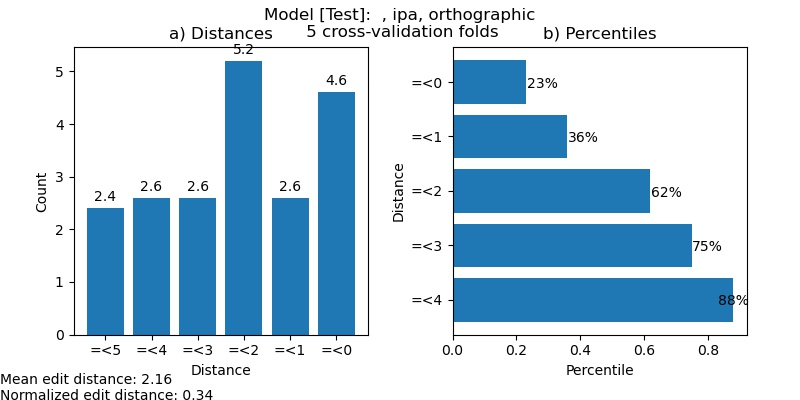
\includegraphics[width=\textwidth]{deep_test_ipa_ortho.jpg}
    \label{fig:sdtio}
\end{figure}

\begin{figure}
    \centering
    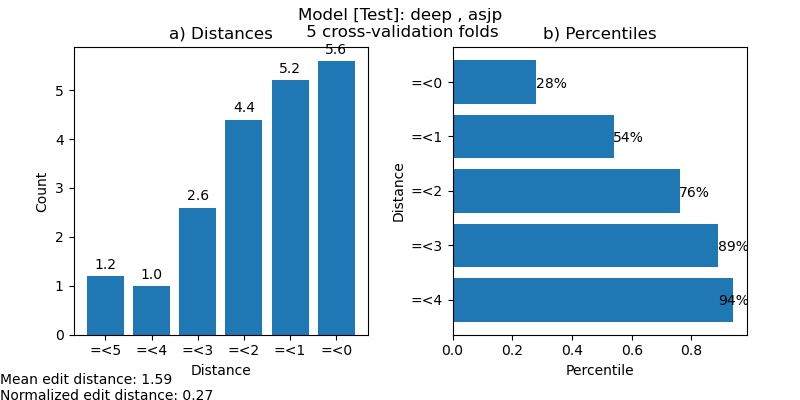
\includegraphics[width=\textwidth]{deep_test_asjp.jpg}
    \label{fig:sdta}
\end{figure}

\begin{figure}
    \centering
    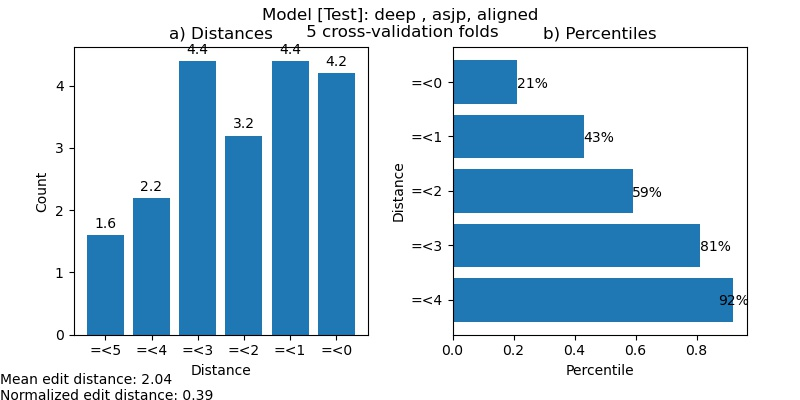
\includegraphics[width=\textwidth]{deep_test_asjp_aligned.jpg}
    \label{fig:sdtaa}
\end{figure}

\begin{figure}
    \centering
    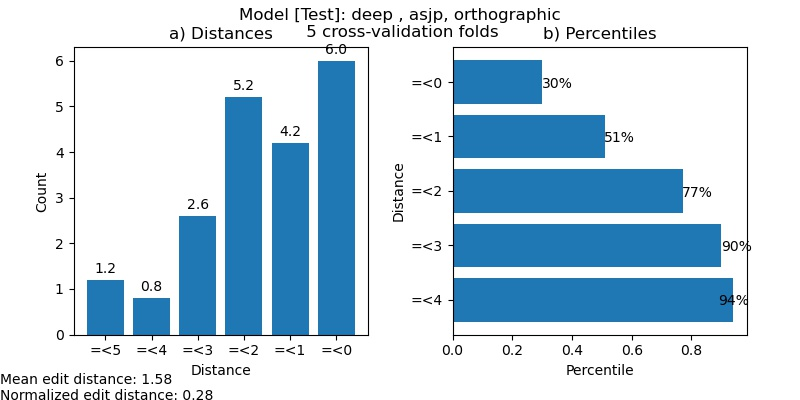
\includegraphics[width=\textwidth]{deep_test_asjp_ortho.jpg}
    \label{fig:sdtao}
\end{figure}

\begin{figure}
    \centering
    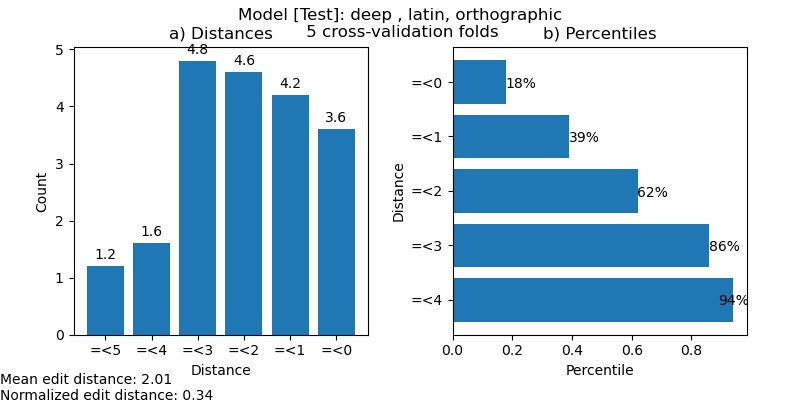
\includegraphics[width=\textwidth]{deep_test_latin_ortho.jpg}
    \label{fig:sdtlo}
\end{figure}

% LSTM, swadesh
\begin{figure}
    \centering
    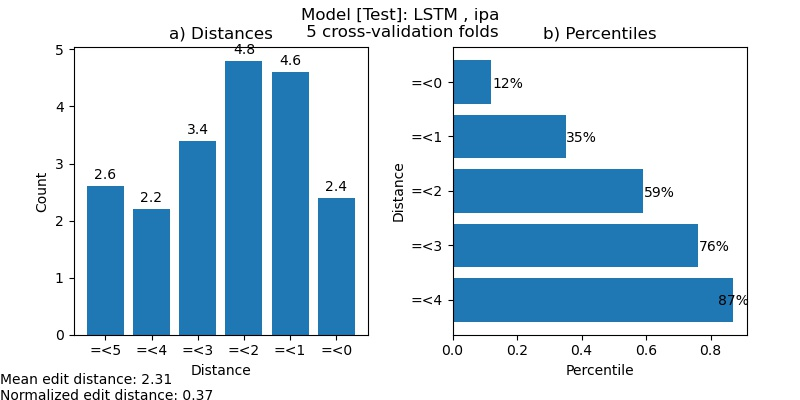
\includegraphics[width=\textwidth]{many2one_test_ipa.jpg}
    \label{fig:smti}
\end{figure}

\begin{figure}
    \centering
    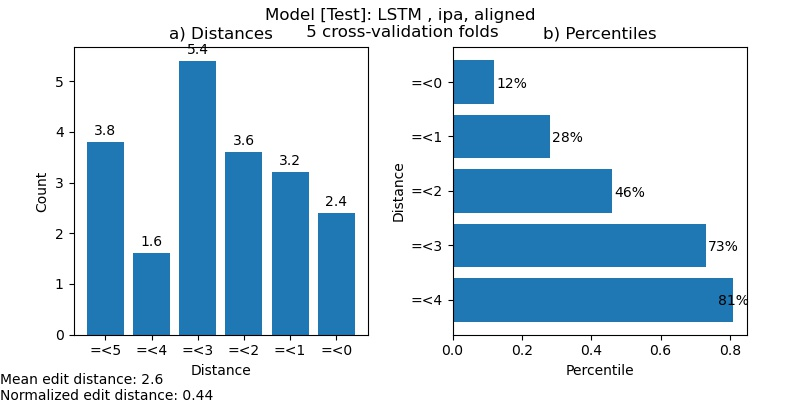
\includegraphics[width=\textwidth]{many2one_test_ipa_aligned.jpg}
    \label{fig:smtia}
\end{figure}

\begin{figure}
    \centering
    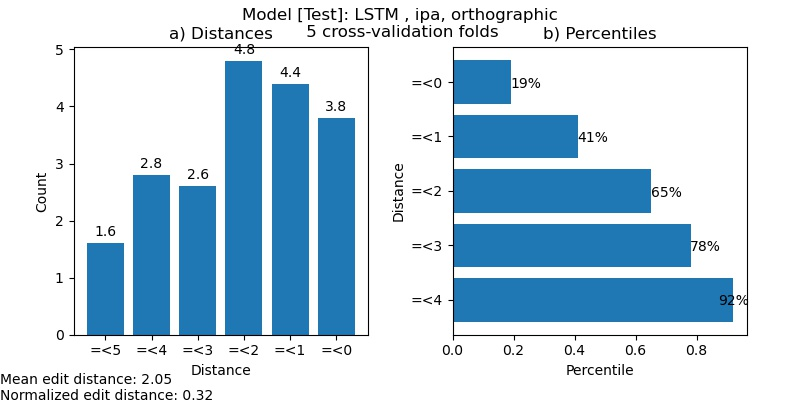
\includegraphics[width=\textwidth]{many2one_test_ipa_ortho.jpg}
    \label{fig:smtio}
\end{figure}

\begin{figure}
    \centering
    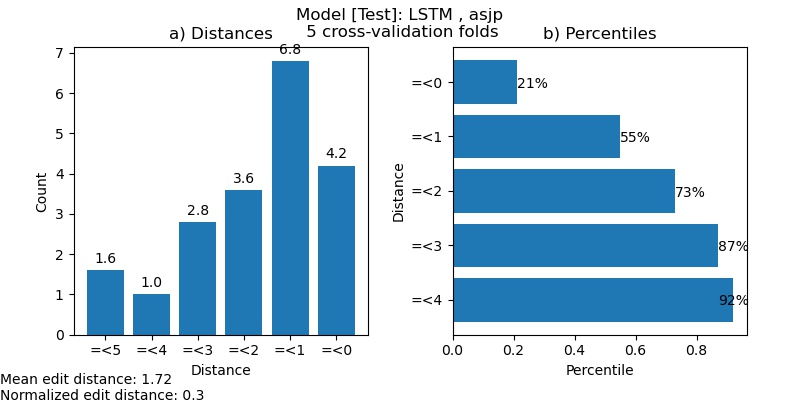
\includegraphics[width=\textwidth]{many2one_test_asjp.jpg}
    \label{fig:smta}
\end{figure}

\begin{figure}
    \centering
    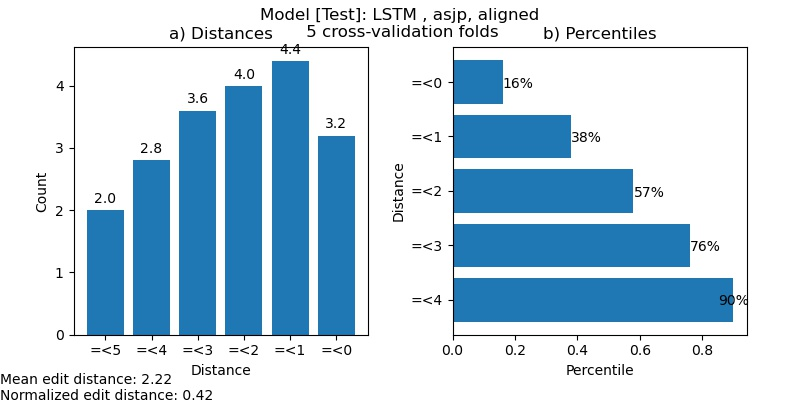
\includegraphics[width=\textwidth]{many2one_test_asjp_aligned.jpg}
    \label{fig:smtaa}
\end{figure}

\begin{figure}
    \centering
    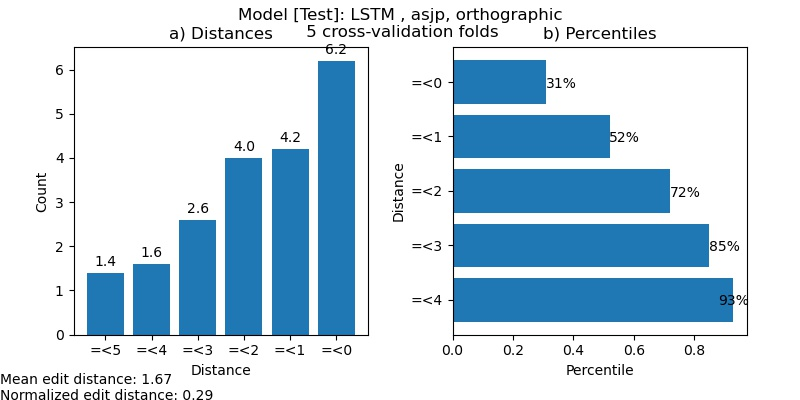
\includegraphics[width=\textwidth]{many2one_test_asjp_ortho.jpg}
    \label{fig:smtao}
\end{figure}

\begin{figure}
    \centering
    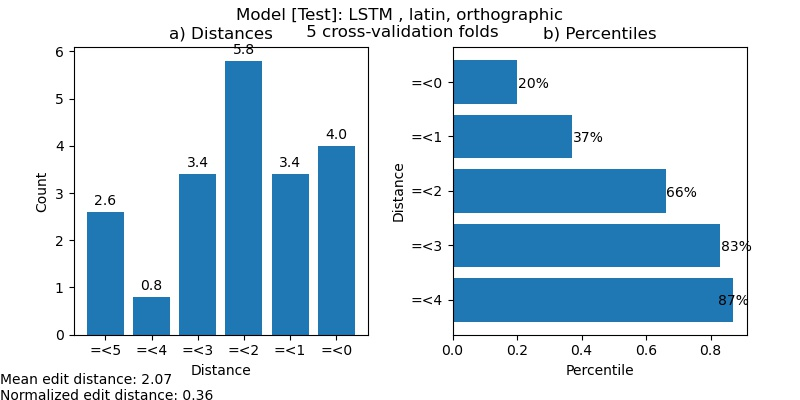
\includegraphics[width=\textwidth]{many2one_test_latin_ortho.jpg}
    \label{fig:smtlo}
\end{figure}

% Deep, Ciobanu
\begin{figure}
    \centering
    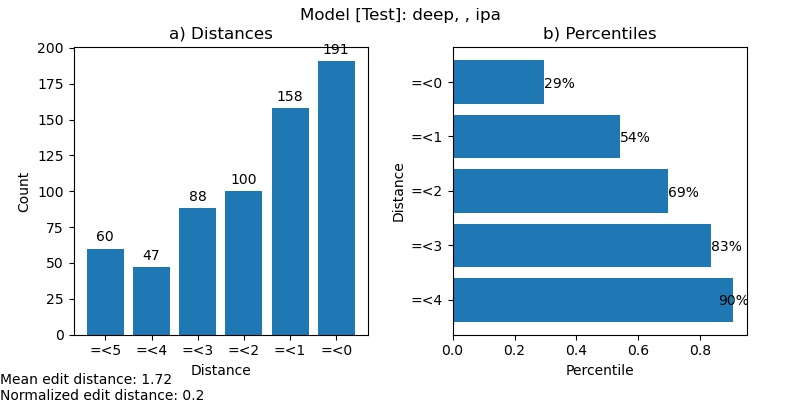
\includegraphics[width=\textwidth]{ciobanu_deep_test_ipa.jpg}
    \label{fig:sdti}
\end{figure}

\begin{figure}
    \centering
    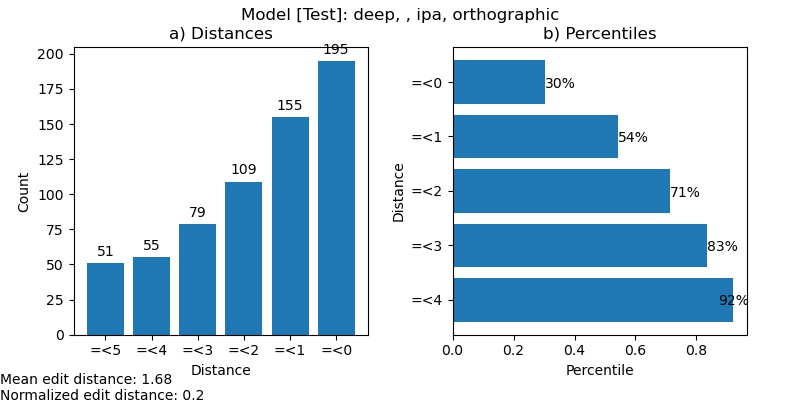
\includegraphics[width=\textwidth]{ciobanu_deep_test_ipa_ortho.jpg}
    \label{fig:sdtio}
\end{figure}

\begin{figure}
    \centering
    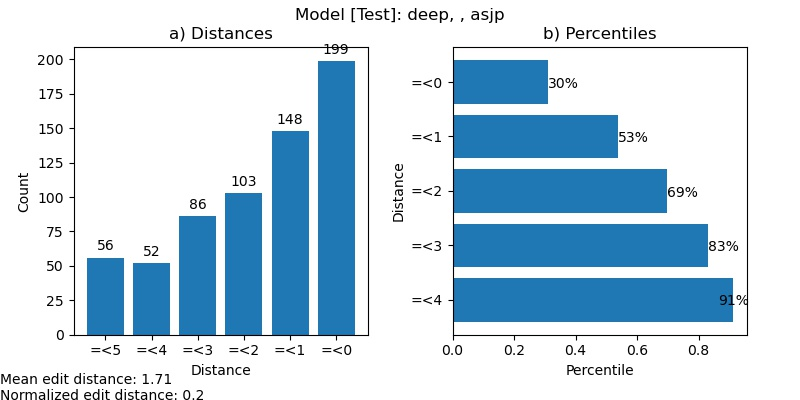
\includegraphics[width=\textwidth]{ciobanu_deep_test_asjp.jpg}
    \label{fig:sdta}
\end{figure}

\begin{figure}
    \centering
    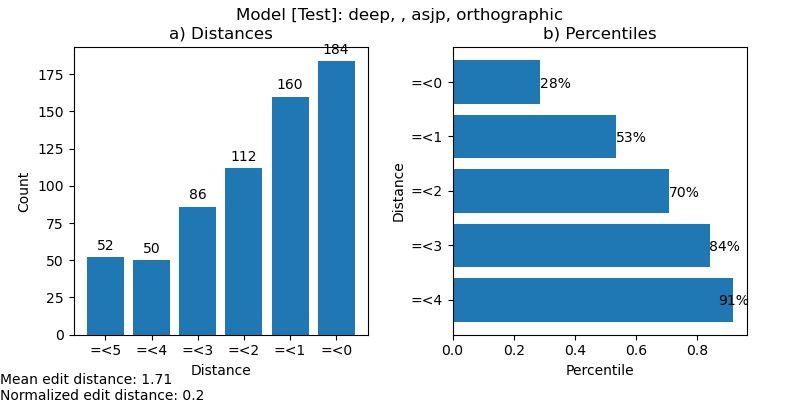
\includegraphics[width=\textwidth]{ciobanu_deep_test_asjp_ortho.jpg}
    \label{fig:sdtao}
\end{figure}

\begin{figure}
    \centering
    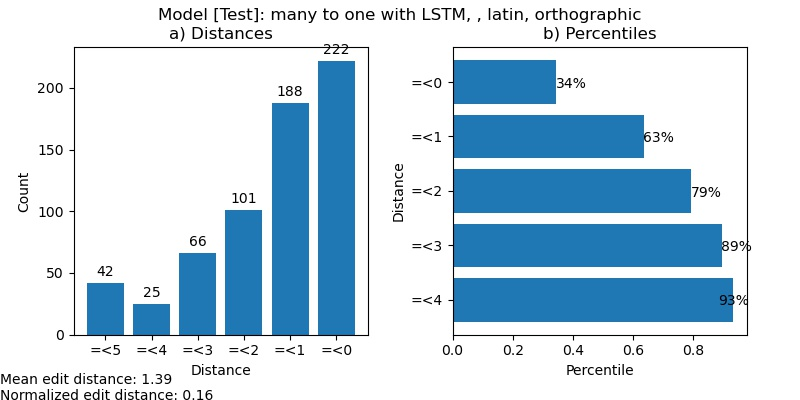
\includegraphics[width=\textwidth]{ciobanu_deep_test_latin_ortho.jpg}
    \label{fig:sdtlo}
\end{figure}

% LSTM, Ciobanu
\begin{figure}
    \centering
    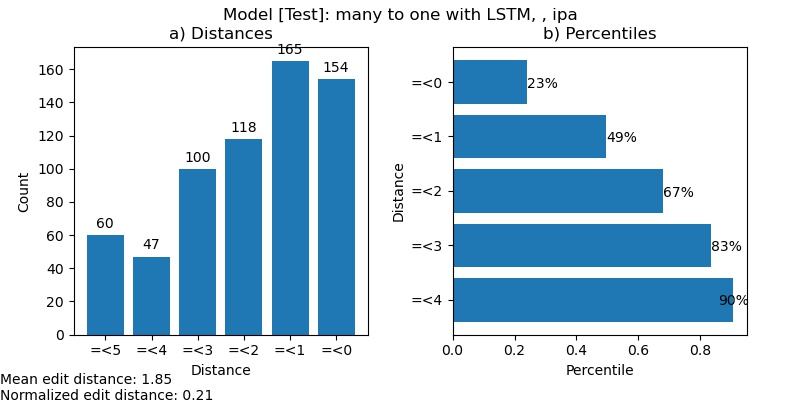
\includegraphics[width=\textwidth]{ciobanu_many2one_test_ipa.jpg}
    \label{fig:sdti}
\end{figure}

\begin{figure}
    \centering
    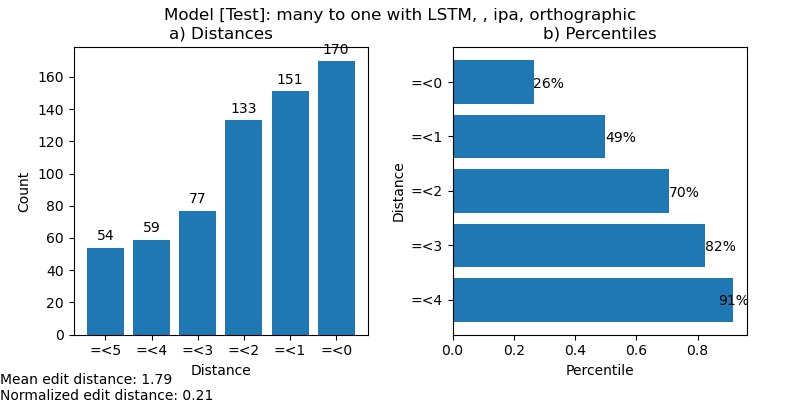
\includegraphics[width=\textwidth]{ciobanu_many2one_test_ipa_ortho.jpg}
    \label{fig:sdtio}
\end{figure}

\begin{figure}
    \centering
    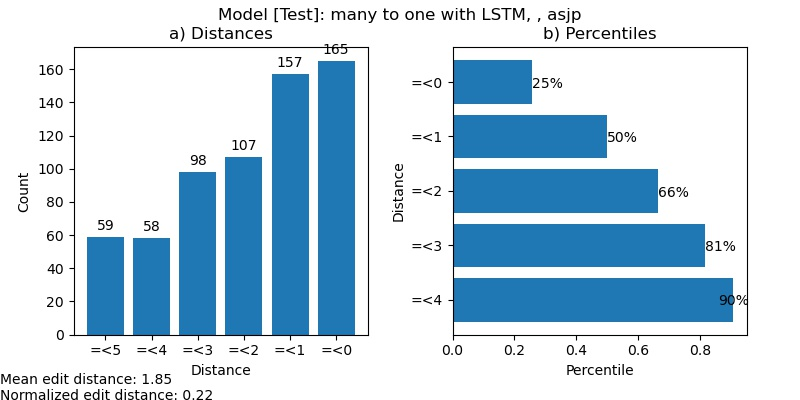
\includegraphics[width=\textwidth]{ciobanu_many2one_test_asjp.jpg}
    \label{fig:sdta}
\end{figure}

\begin{figure}
    \centering
    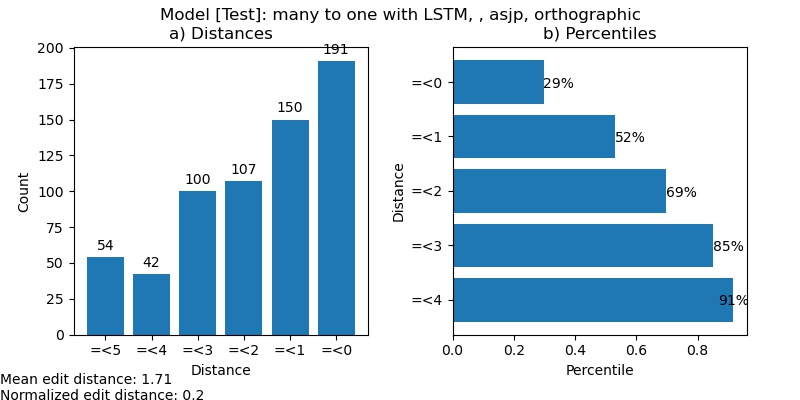
\includegraphics[width=\textwidth]{ciobanu_many2one_test_asjp_ortho.jpg}
    \label{fig:sdtao}
\end{figure}

\begin{figure}
    \centering
    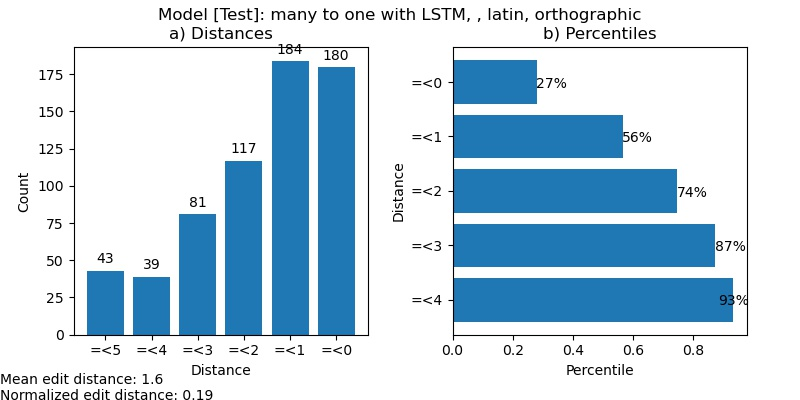
\includegraphics[width=\textwidth]{ciobanu_many2one_test_latin_ortho.jpg}
    \label{fig:sdtlo}
\end{figure}
%-----------------------------------------------------------------------------------------------------
%--- Discussion
%-----------------------------------------------------------------------------------------------------
\section{Discussion}
The choice of alphabet seems to have the largest impact on reconstruction accuracy. Similar to \citet{meloni2019ab} both models performed worse on the IPA transcriptions across both datasets. One reason for this might be that there are more features encoded in the IPA than in the ASJP.
We assume that the overall better performance on the Latin orthographic data is because of the etymological information contained in, e. g., the french orthography. The overall higher reconstruction accuracy on dataset \textbf{II} may be caused by its larger size (3128 items versus 100 in dataset \textbf{I}) and it containing a large portion of direct loans from Latin.
To our surprise both models fared almost equally well with either dataset, with a small advantage for the feedforward model (\textbf{B}) observable with dataset \textbf{II}. This result should be more reliable because of the larger size of dataset \textbf{II}. This indicates that the higher accuracy scores in both \citet{ciobanu-dinu-2018-ab} and \citet{meloni2019ab} are indeed due to the decoder-encoder architecture with attention, which makes the machine translation pipeline a plausible choice for the task of proto-word reconstruction. However, the poor performance of both our models on the Swadesh list data in dataset \textbf{II} demonstrates that this approach relies on a high number of cognate sets being available to the researcher, which cannot be expected to be the case for language families for which no literary records and therefore no direct information about the proto language is present, e. g. the Papuan clades.
 
 %BIG DRAWBACK: We should test the small dataset with Ciobanu's and Meloni's original pipeline, else it doesn't make much sense to %directly compare the results. Not time for that now, but since the deadline is November 27 and that's something we certainly will %get as feedback we can do that after the project deadline. Also will be a good preparation for your transformer seminar;)
 
%-----------------------------------------------------------------------------------------------------
%--- Conclusion
%-----------------------------------------------------------------------------------------------------
\section{Conclusion}
In this paper we reproduced the result of prior studies that more fine-grained encodings presents a challenge for recontruction models. Our results also indicate that a machine-translation-like decoder-encoder architecture may be necessary to achieve high accruracy scores for datasets comparable to \citet{ciobanu-dinu-2014-automatic}. On the other hand we assume that the poor model performance on our self-compiled dataset constitutes an inherent problem to the automated reconstruction of proto-words: 
if large cognate datasets are required to achieve an acceptable level of reconstruction accuracy, relying on small datasets to automatically reconstruct proto-words may be impossible. To verify this hypothesis we want to apply the architecture used by \citet{meloni2019ab} on our dataset.
% That last sentence is not good


%\section{Final Thoughts}
%maybe this section should be titled future work instead




%\section*{Acknowledgments}

%The acknowledgments should go immediately before the references. Do not number the acknowledgments section.
%Do not include this section when submitting your paper for review.

\newpage
\input{section2}


% REFERENCES
\newpage
\bibliographystyle{apalike}
\bibliography{references,anthology}

\end{document}